\documentclass{article}
\usepackage{graphicx} % Required for inserting images
\usepackage{amsmath,amssymb}
\usepackage{enumerate}
\usepackage{dcolumn}
\usepackage{bm}
\usepackage{microtype}
\usepackage{xcolor}


\definecolor{navyblue}{rgb}{0.0, 0.0, 0.5}
\usepackage{hyperref}
\usepackage{cleveref} 
\hypersetup{
    colorlinks=true,
    linktoc=all,
    allcolors=navyblue
}

\bibliographystyle{ieeetr}

\title{Axiverse Machine}
\author{Masha Baryakhtar, David Cyncynates, Ella Henry}
\date{\today}

\begin{document}

\maketitle
\section{Anthropics}
The bounds for the possible ratio of the dark matter abundance to baryon abundance, $\zeta$, are given in \cite{anthropic-explanation} to be $2.5<\zeta <100$. The lower bound is related to the value for which perturbations near the size of our galaxy's stop growing, and the upper bound is related to the value that ultimately prevents star formation. All values within this range are allowed in the sense that they would lead to our existence today, but their likelihoods depend on the theory for dark matter, as we will see below. In section 5 of \cite{exploring-string-axiverse}, the authors consider the case of $n$ axions and the fraction of the dark matter that they constitute. If the axions make up all of the dark matter, then we can write $\zeta$ as:

\begin{equation}
\label{eq:zeta}
    \zeta = \sum_{a=1}^n c(m_a) F(\theta_a)
\end{equation}

Here, $c(m_a)F(\theta_a)$ is the fractional abundance in the $a$-th axion, where $F(\theta_a)$ encodes the dependence of the fractional abundance on the axion's intial misalignment angle. For small enough angles, $F(\theta_a)\sim\theta_a^2$. The $c(m_a)$ factor takes into account the fractional abundance's dependence on the mass and on the scale of symmetry breaking, e.g. for axions that start to oscillate during radiation domination, $c(m_a) \sim \Big(\frac{m_a}{H_{eq}}\Big)^{1/2}\Big(\frac{f_a}{M_{pl}}\Big)^2$.

\subsection{The anthropic measure}

The authors of \cite{exploring-string-axiverse} then calculate the probability $P$ of finding ourselves in a causal patch where the dark matter abundance is no larger than the observed value of $\zeta \sim 5$, without being so small that we could not exist, in other words, the probability that $2.5<\zeta<5$. The calculation uses the causal diamond measure (details in \cite{anthropic-explanation}) to circumvent the problem of computing probabilities in an infinite-dimensional space, which leads to difficulties in normalizing these probabilities. The measure allows us to restrict ourselves to one causal patch and consider the number of observations made in that patch. To determine this number, the author of \cite{anthropic-explanation} counts the number of baryons in a causal patch and then the number of observations per baryon. The quantitative expression the author finds for the number of baryons in a causal patch is $(1+\zeta)^{-1}$ with the assumption of fixed baryon-to-photon ratio. The number of observers per baryon is approximated to be constant within the range of allowed $\zeta$ values. The overall contribution to the probability density from the causal diamond measure is therefore $C(1+\zeta)^{-1}$, for some constant $C$.

We must also assume some distribution for the initial conditions $theta_a$, which will depend on the scale of inflation relative to the axion's potential: for high scale inflation, the distribution is flat between $[-\pi,\pi]$, while for low scale inflation,     $p(\theta_a) \propto \exp{\left(-\frac{8\pi^2V(\theta_a)}{3H^4}\right)}$, where $V(\theta_a)=\Lambda^4(1-\cos{\theta_a})$. We can approximate this distribution from low scale inflation as flat between $[-\sigma,\sigma]$, where $\sigma^2 = 3H^4/(8\pi^2m^2f^2)$ is the spread in this distribution. So in general, we can consider $p(\theta_a)$ as flat between two values, which we'll call $\pm f(H)$, where:

\begin{equation}
\label{eq:f(H)}
    f(H) = \begin{cases}
        \pi \; \text{ for } H>\Lambda\\
        \sigma \; \text{ for } H < \Lambda
    \end{cases}
\end{equation}

Now, using the causal diamond measure described above and the flat distribution between $\pm f(H)$ for the initial conditions, we can write down an expression for the probability $P$:

\begin{equation}
    \label{eq:prob-deriv}
    P = N^{-1} \frac{C}{(2f(H))^n}\int_{2.5<\zeta(\theta_a)<5} \frac{\prod_{a=1}^nd\theta_a}{1+\zeta(\theta_a)}
\end{equation}

\noindent where again $n$ is the number of axions and $C$ is the constant factor from the number of observations per baryon. The normalization $N$ is such that the probability is normalized to 1 and is given by:

\begin{equation}
    \label{eq:prob-deriv-norm}
    N = \frac{C}{(2f(H))^n}\int_{2.5<\zeta(\theta_a)<100} \frac{\prod_{a=1}^nd\theta_a}{1+\zeta(\theta_a)}
\end{equation}

We can compute this probability for any value of $f(H)$ by rescaling the integration variables as $\theta_a' = \theta_a/f(H)$ and writing $\zeta(\theta_a)=c_a\theta_a^2$ (summing over the $a$ index):

\begin{equation}
    \label{eq:general-prob}
     P = \mathcal{N}^{-1} \int_{-1}^1 \frac{\prod_{a=1}^nd\theta_a'}{1+c_a'\theta_a'^2}\Theta(c_a'\theta_a'^2-2.5)\Theta(5-c_a'\theta_a'^2)
\end{equation}

\noindent where the $\theta_a$-independent factors out front in Eq. \eqref{eq:prob-deriv} have canceled out with those in the normalization $N$, and so $\mathcal{N}$ is the same as $N$, without those factors. $\Theta$ here is the Heaviside function and $c_a'\equiv c_af(H)^2$.

\subsection{1 axion}

The probability for one axion can be computed numerically as a function of $c_1$ and is shown below.

\begin{figure}[h]
    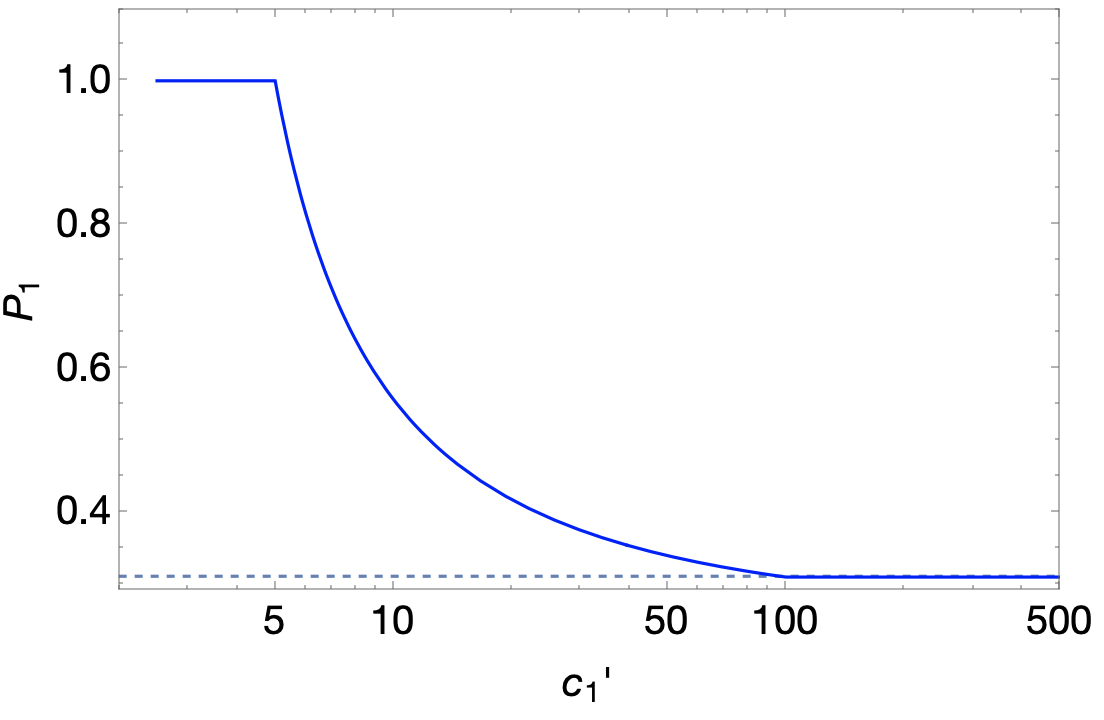
\includegraphics[scale=0.5]{figs/1axion-prob.jpeg}
    \centering
    \caption{Probability of measuring $2.5<\zeta<5$ in the case of one axion, as a function of $c_1'$. The dashed horizontal line corresponds to $P=0.3$, the probability found for 1 axion in \cite{exploring-string-axiverse}}.
    \label{fig:1axion-prob}
\end{figure}

Fig. \ref{fig:1axion-prob} shows that once $c_1'>\zeta_\text{upper}=100$, the probability becomes independent of the axion parameters (recall that $c' \propto m^{1/2}f^2$), and acquires the constant value of $P=0.3$. This corresponds to the $n=1$ case of the result presented in Eq. 79 of \cite{exploring-string-axiverse}, reproduced below:

\begin{equation}
\label{eq:bookkeeping-result}
    P_n = \frac{\int_{2.5}^5 \frac{d\zeta \zeta^{(n-2)/2}}{1+\zeta}}{\int_{2.5}^{100}\frac{d\zeta \zeta^{(n-2)/2}}{1+\zeta}} = \text{0.3, 0.16, 0.06, 0.02, 0.006, . . .}
\end{equation}

\noindent In this result, the authors focus on $n$ axions at the GUT scale ($f\sim 10^{16}$ GeV), with masses heavy enough ( $m_a\geq10^{-19}$ eV) so that the axions would find themselves in this constant $P$ regime. Indeed, one can check that for $f\sim 10^{16}$ GeV and $m_a\geq10^{-19}$ eV, the criterion $c_a>100$ is satisfied.

\subsection{2 axions}

We can compute the probability in Eq. \eqref{eq:general-prob} now for $n=2$, numerically, and plot the results as a function of $c_2'$, for a few chosen values of $c_1'$. This is shown below in Fig. \ref{fig:2axion-prob}

\begin{figure}[h]
    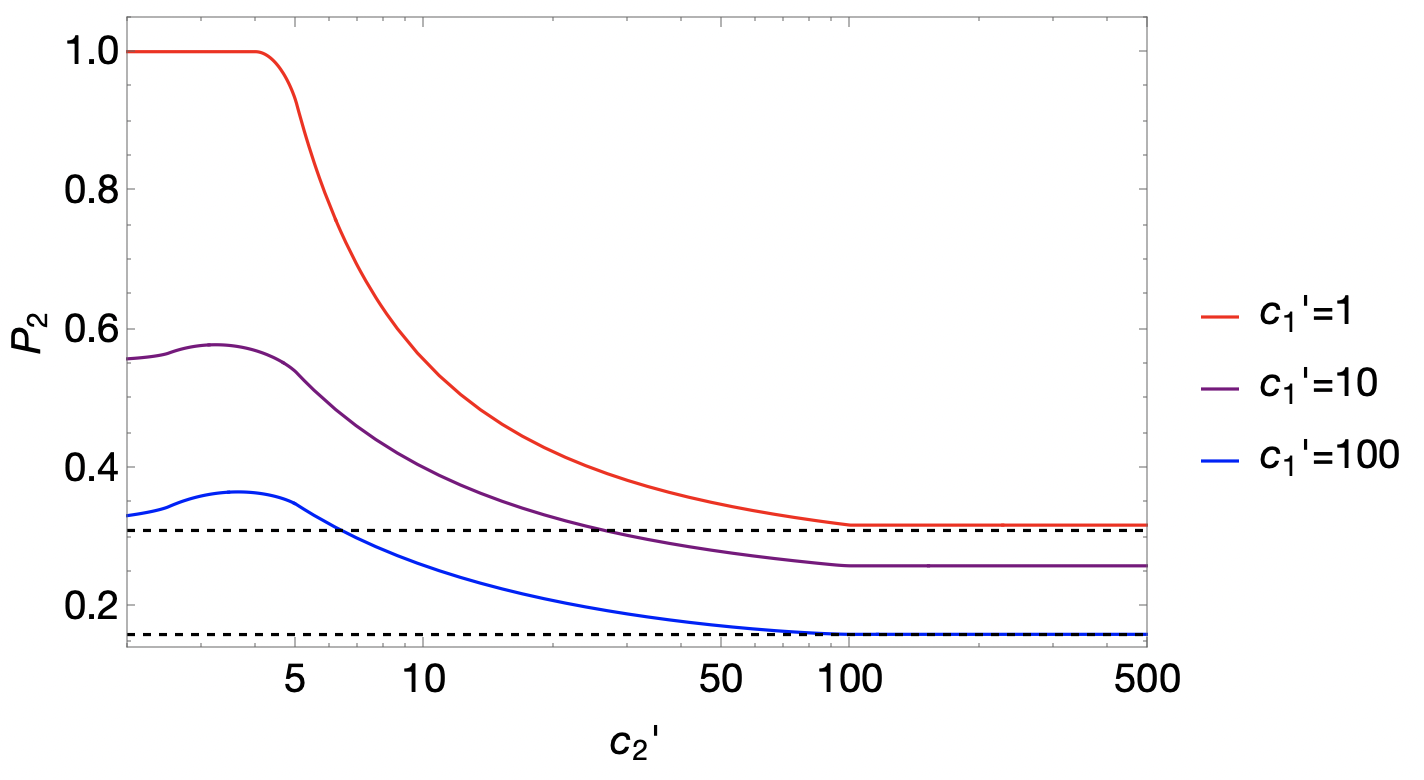
\includegraphics[scale=0.5]{figs/2axion-prob.jpeg}
    \centering
    \caption{Probability of measuring $2.5<\zeta<5$ in the case of two axion as a function of $c_2'$, for different values of $c_1'$. The dashed horizontal lines correspond to the probabilities for 1 and 2 axions as given by Eq. \eqref{eq:bookkeeping-result}: 0.3 and 0.16 respectively.}.
    \label{fig:2axion-prob}
\end{figure}

The behavior of $P_2$ shows that there is a little more nuance, but the result that an axion contributes to the anthropic measure once $c'>\zeta_\text{upper}$ holds true. We see that if $c_1'\ll\zeta_\text{upper}$ and $c_2'>\zeta_\text{upper}$ (see red line for larger $c_2'$ in Fig. \ref{fig:2axion-prob}), the the first axion does not contribute while the second one does, and thus we recover the $P=0.3$ probability from the 1-axion scenario. The same is true if $c_1'>\zeta_\text{upper}$ and $c_2'\ll\zeta_\text{upper}$ (Fig. \ref{fig:2axion-prob}, blue line for small $c_2'$). If both $c_1',c_2'>\zeta_\text{upper}$ (Fig. \ref{fig:2axion-prob}, blue line for large $c_2'$), then the two axions contribute to the measure and so the probability is $P=0.16$, in agreement with Eq. \eqref{eq:bookkeeping-result}. There is a weird middle regime (purple line in Fig. \ref{fig:2axion-prob}, as well as region in all three lines where there is a bump), where I am not really sure what's going on yet. 

We have thus seen, in the case 1 and 2 axions, that the condition that an axion must satisfy to contribute to the anthropic measure is $c'>\zeta_\text{upper}$. Recalling that $c'=c\,f(H)^2$ (with $f(H)$ given in Eq. \eqref{eq:f(H)}), and that $c=(m/H_{eq})^{1/2}(f/M_{pl})^2$ we can write this condition in terms of the physical parameters as:

\begin{equation}
    \label{eq:c-condition}
    \boxed{\left(\frac{m}{H_{eq}}\right)^{1/2}\left(\frac{f}{M_{pl}}\right)^{2}\min{ \Bigl\{ \pi^2,\frac{3H^4}{8\pi^2m^2f^2}\Bigr\}}>\zeta_\text{upper}}
\end{equation}

The takeaway is that if the scale of inflation is low, heavier axions will evade this criterion and therefore will not contribute to the anthropic measure: including them in the theory does not require more fine-tuning. On the other hand, if the scale of inflation is high, these axions will quickly satisfy this condition and require fine-tuning, while lighter axions won't (the words ``lighter" and ``heavier" depend on the values of $H$ and $f$ in each case respectively; this will need to be further investigated).

Note that Eq. \eqref{eq:c-condition} is approximate in that: (1) it assumes that $F(\theta_a)\sim\theta^2$, which is not true if $\theta_a \sim O(1)$, in which case there is a small correction; (2) it approximates the distribution of $\theta_a$ in a low scale inflation scenario to be flat between $\pm \sigma$, instead of treating it fully as $\propto \exp{\left(-V(\theta_a)/H^4\right)}$; and (3) it only accounts for regimes where $H<\Lambda$ or $H>\Lambda$, and glosses over the $H\sim\Lambda$ regime.

\subsection{Exact anthropic probability with low scale inflation}

In the previous section, we used an approximate form for the distribution of initial conditions from low scale inflation. We can compute the anthropic probability \textit{for one axion} more precisely in the case of low scale inflation by numerically calculating the following:

\begin{equation}
    \label{eq:inflation-prob-1axion}
    P = N^{-1}\int_{2.5<\zeta<5} \frac{d\theta}{1+\zeta} \exp{\left(-\frac{8\pi^2V(\theta)}{3H^4}\right)}
\end{equation}

\noindent where the normalization is the same integral but with integration bound $2.5<\zeta<100$. This probability is plotted against $\sqrt{mf}$ for certain values of $H$ in Fig. \ref{fig:low-scale-inf-prob} (and $f$ is set to 1).

\begin{figure}[h]
    \centering
    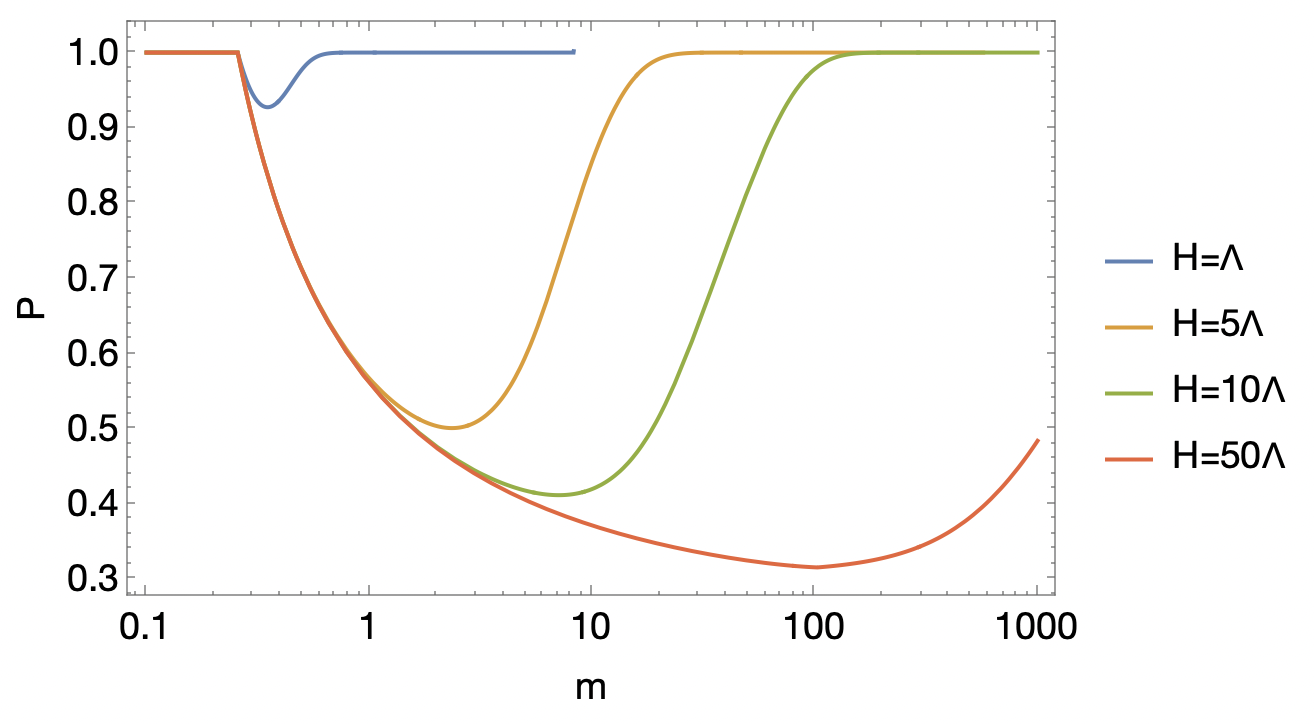
\includegraphics[width=1\linewidth]{figs/low-scale-inf-prob.jpeg}
    \caption{Probability of $2.5<\zeta<5$ for a stochastic axion scenario (low scale, long-lasting inflation), with different vales of $H$ relative to $\Lambda = (mf)^{1/2}$. In this plot, $f=1$.}
    \label{fig:low-scale-inf-prob}
\end{figure}

As expected, for each curve, we see that when the scale of inflation is low relative to the size of the potential (i.e. $H<\Lambda$), the probability that $2.5<\zeta<5$ grows, since you are sampling $\theta$ from a distribution peaked closer and closer to zero (effectively acts like a small $c$). When $H>\Lambda$, you recover the expected behavior from flat initial conditions: the probability drops for $\Lambda$ (until $\Lambda \sim H$, and then you enter the first regime). \\

\color{red}\noindent \textbf{Things to do:}
\begin{enumerate}
    \item could include correction to the energy density from cosine potential in the probability calc
    \item what happens below $c=\zeta_\text{upper}$?
    \item and related to the previous point, what is the bump? what does it looks like with more axions?
    \item visualize/better understand the parts of parameter space that are viable via anthropics using Eq. \eqref{eq:c-condition}
    \item keep in mind dependence of results on choice of measure (causal diamond vs others?)
\end{enumerate}\color{black}

\section{GSification}

\appendix
\section{Introduction}
Consider the general task of determining how the initial condition of a collection of scalar fields $\bm \theta(0)$ maps onto the final partition of energy density among the various mass eigenstates, where the dynamics are controlled by the following Lagrangian:
\begin{align}\label{eqn:fundamental}
    {\cal L} = \frac{1}{2}\dot{\bm \theta}^T {\bm K}\dot{\bm\theta} - V(\bm\theta)\,.
\end{align}
The kinetic term matrix $\bm K$ may be diagonalized through the following field redefinition
\begin{align}
    \bm\psi \equiv \bm F \bm R^T \bm\theta\,,\hspace{1cm}\bm F^2\equiv \bm R^T \bm K \bm R\,,
\end{align}
where $\bm R^T \bm R  = 1$, and $\bm F^2$ is the diagonal matrix of $\bm K$ eigenvalues. In this basis, the Lagrangian becomes
\begin{align}\label{eqn:canonical}
    {\cal L} = \frac12\dot{\bm\psi}^T\dot{\bm\psi} - V(\bm R\bm F^{-1}\bm\psi)\,.
\end{align}
Although one may as well have started with \Cref{eqn:canonical}, starting with \Cref{eqn:fundamental} is essential if the form of $V$ is specified, since mixing induced by the off-diagonal kinetic terms will play an important role in the dynamics.

The potential $V(\bm\psi)\equiv V(\bm R\bm F^{-1}\bm\psi)$ is in general an arbitrarily complicated function of the fields, and it may have multiple, physically inequivalent minima, from which $\bm\psi$ may be initialized arbitrarily far away. Therefore, at early times there is no sense in which one may define any particular linear combination of the fields to carry some definite fraction of the energy density of the system. Only at asymptotically late times is one guaranteed that the fields settle into a local minimum of the potential, though I emphasize that one does not know the location or curvature of this part of the potential \emph{a priori}. Therefore, our algorithm to separate out the various late-time mass eigenstates of the fields must avoid making explicit reference to the shape of the potential about any particular point.


\subsection{Separable energy density}\label{sec:separable-energy-density}
To simplify notation, we will use $\bm V''$ and $\bm V'$ to refer to the second and first derivatives $\partial^2 V(\bm\psi)/\partial\bm\psi\partial\bm\psi$ and $\partial V(\bm\psi)/\partial\bm\psi$ respectively. The matrix $\bm V''$ defines the square of the local mass eigenvalues, and so we must redefine the fields to work in the mass eigenstates:
\begin{align}
    \bm\phi\equiv \bm S^T\bm\psi \,,\hspace{1cm} \bm M^2\equiv \bm S^T\bm V''(\psi)\bm S\,,
\end{align}
where $\bm S^T\bm S = 1$ and $\bm M^2$ is the diagonal matrix of $\bm V''(\psi)$ eigenvalues. The energy density contained in the field oscillations is then
\begin{align}
    \rho_{\rm tot}\equiv \frac12 \dot{\bm\phi}^T\dot{\bm\phi} + \frac12 (\bm\phi - \bm\phi_0)\bm M^2(\bm\phi - \bm\phi_0)\,,
\end{align}
where $\bm\phi_0$ is the location of the minimum of the potential, which approximately satisfies
\begin{align}
    0&=\bm V''(\bm\psi)(\bm \psi - \bm\psi_0) + \bm V'(\psi) = \bm S \bm M^2 (\bm\phi - \bm \phi_0) + \bm S\bm V'(\bm\phi)
\end{align}
Thus, the energy density is
\begin{align}
    \rho_{\rm tot}\equiv \frac12 \dot{\bm\phi}^T\dot{\bm\phi} + \frac12\bm V'(\bm\phi)^T\bm M^{-2}\bm V'(\bm\phi)\,.
\end{align}
Labeling each of the mass eigenstates by their mass eigenvalue $m$, we may decompose the energy density:
\begin{align}\label{eqn:separated-energy-densities}
    \rho_{m}\equiv \frac12 \dot{\bm\phi}_m^2 + \frac12 [\bm M^{-2}(\bm V'(\bm\phi))^2]_m\,.
\end{align}
I assume a convention where the modes are sorted from lightest to heaviest, with $m = m_0$ being the lightest eigenvalue and $m_{-1}$ the heaviest.

\subsection{Pruning trivial modes}
The procedure of \Cref{sec:separable-energy-density} is sufficient to determine the final partition of energy densities at asymptotically late times. In practice, integrating the equations of motion to very late times where one may assume that all states have settled to the bottom of some local minimum is impossible if the masses span more than a few orders of magnitude, since the number of time steps that must be taken is proportional to the ratio of the largest to smallest masses. On the other hand, heavy particles will settle to the minimum of their potential long before the lightest mass eigenstates have begun to oscillate, and so we may remove them from the integration by carefully checking that these modes are dynamically decoupled from all others.

To eliminate the heavy modes, it is enough to replace the damping term $3 H \dot{\bm \phi}_{m_i}$ with the critically damped term $2m_i\dot{\bm \phi}_{m_i}$. Note, though, that at every step, the heavy modes will still involve the heavy mass scale. Therefore, one should re-scale the heavy-mode EOM by the mass (squared) of the lightest mode that has been integrated out. This will keep the heavy modes dynamically forced to the bottom of their potentials, while removing any fast timescales.

\section{Coupling to photons}
In the interaction basis, there is a single mode that couples to photons, which we take to be $\theta_1$ without loss of generality:
\begin{align}
    {\cal L}_{\rm int} = \frac{\alpha_{\rm EM}}{8\pi}\theta_1\tilde F F =\frac{\alpha_{\rm EM}}{8\pi} [\bm R\bm F^{-1}\bm S \bm \phi]_1 \tilde F F.
\end{align}
For each mass eigenstate, the coupling to the photon is then given by the corresponding coefficient in the first row of this matrix.

\begin{figure}
    \centering
    \includegraphics[width=1\linewidth]{figs/Screenshot 2024-11-12 at 5.53.04 PM.png}
    \caption{This is a simulation of the trivial case where each axion has its own instanton and the kinetic term is diagonal. The blue line represents the expectation that $\rho\propto m^{1/2}$. The horizontal axis is the log of the masses normalized against some arbitrary mass scale, while the vertical axis is the asymptotic relic abundance of each mass eigenstate normalized against some arbitrary energy density.}
    \label{fig:enter-label}
\end{figure}
\begin{figure}
    \centering
    \includegraphics[width=1\linewidth]{figs/Screenshot 2024-11-12 at 5.53.09 PM.png}
    \caption{40 axions!}
    \label{fig:enter-label}
\end{figure}
\begin{figure}
    \centering
    \includegraphics[width=1\linewidth]{figs/Screenshot 2024-11-12 at 5.53.14 PM.png}
    \caption{20 axions!}
    \label{fig:enter-label}
\end{figure}

\section{Directions}
\begin{enumerate}
    \item Plot: $g_{a\gamma\gamma}\sqrt{\rho/\rho_{\rm DM}}$ vs mass (like what we have in the friendship paper) for all the axions.
    \item Theoretical expectation for thermalization rate of nonlinearly coupled chain of oscillators -- extend to time-varying parameters with adiabatic approximation
    \item Theoretical expectations for the distribution of energy density among the mass eigenstates
    \item Effect of QCD Axion?
    \item Statistics of the CC (what is the distribution of vacuum energies?)
\end{enumerate}

\section{Being more clever}
Let us consider the algorithm more carefully, and consider how it may be improved.
\begin{enumerate}
    \item Heavy modes are still kept. Can we drop them entirely using an analytical method without introducing numerical error? Perhaps we simply don't include them in the rotation matrix?
    \item Light modes are included in the rotation matrix even though they don't need to be included. Perhaps only including the oscillating modes in the rotation matrix would improve numerical stability.
    \item In order to avoid using arbitrary precision during numerical integration, consider why arbitrary precision may be considered necessary at all. It is only the case that arbitrary precision would be necessary if terms with a huge dynamical range entered into the light field equations of motion in the first place. These terms necessarily cancel -- how can we eliminate them without losing precision? IDEA: Suppose there are N dynamical degrees of freedom -- using arbitrary precision, precompute an N dimensional subvolume of the potential
\end{enumerate}

\bibliography{refs}

\end{document}
